\section{The lens \protect
\includegraphics[height=1em]{figs/microscope.png}: Agent evaluation with AutoLibra}
\label{sec:lens}

In this section, we use AutoLibra as a lens to provide insights into agent behaviors. We first try to validate
the steps of AutoLibra by annotating the 

\begin{wrapfigure}[8]{r}{0.5\textwidth}
    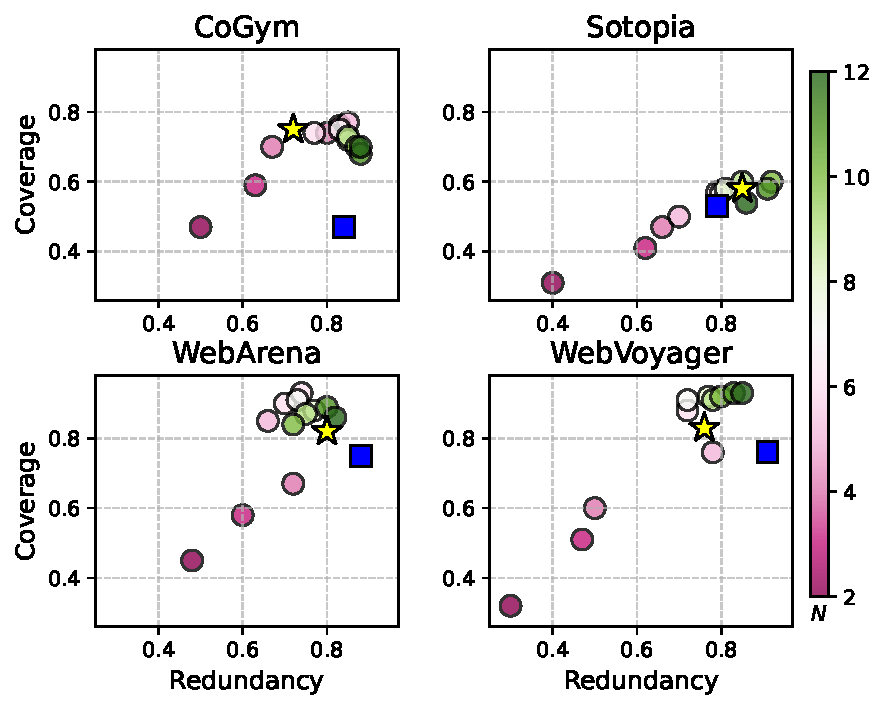
\includegraphics[width=0.5\textwidth]{figs/four_datasets_grid.pdf}
\end{wrapfigure}

\subsection{Are LLMs aligned with human judgment in AutoLibra?}



\subsection{How do AutoLibra metrics compare with human-derived metrics?}



\subsection{Are examples in the metrics useful for LLM-as-a-Judge?}

